% ------------------------------------------------------------------------------
% TYPO3 CMS 7.4 - What's New (English Version)
%
% @author	Michael Schams <schams.net>
% @license	Creative Commons BY-NC-SA 3.0
% @link		http://typo3.org/download/release-notes/whats-new/
% @language	English
% ------------------------------------------------------------------------------
% LTXE-CHAPTER-UID:		0dbe76ce-5948c314-454b95fd-543cb62c
% LTXE-CHAPTER-NAME:	Backend Gebruikersinterface
% ------------------------------------------------------------------------------

\section{Backend Gebruikersinterface}

% ------------------------------------------------------------------------------
% LTXE-SLIDE-START
% LTXE-SLIDE-UID:		e71b9ffa-021791bd-994bb6e2-fd89fb9a
% LTXE-SLIDE-ORIGIN:	464d4ba6-dab07499-0cd5f168-552e9729 English
% LTXE-SLIDE-ORIGIN:	8080f469-3c5592f0-dc25ad87-894c2648 German
% LTXE-SLIDE-TITLE:		Feature: #48947 - Avatars for backend users
% LTXE-SLIDE-REFERENCE:	Feature-48947-AvatarsForBackendUsers.rst
% ------------------------------------------------------------------------------
\begin{frame}[fragile]
	\frametitle{Backend Gebruikersinterface}
	\framesubtitle{Avatars voor Backend-gebruikers}

	Om de gebruikerservaring bij het gezamenlijk bewerken van content te verbeteren, kunnen gebruikers
	avatars gebruiken. Deze kleine afbeeldingen zijn te zien in de balk bovenaan, de gebruikerslijst
	en andere plaatsen.

	\begin{figure}
		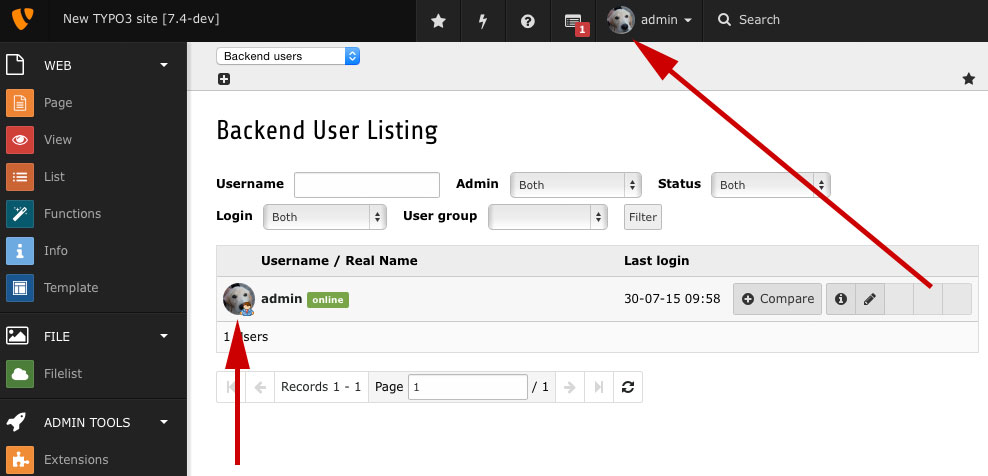
\includegraphics[width=0.9\linewidth]{BackendUserInterface/48947.jpg}
	\end{figure}

\end{frame}

% ------------------------------------------------------------------------------
% LTXE-SLIDE-START
% LTXE-SLIDE-UID:		8a751845-a9459bdd-3e74f91b-f9f633b2
% LTXE-SLIDE-ORIGIN:	89f348c8-db045eff-5dfc4f42-da1a2cfa English
% LTXE-SLIDE-ORIGIN:	b0f7e15a-7cc72aaa-79738ec7-643c5cec German
% LTXE-SLIDE-TITLE:		Feature: #56133 - Replace file feature for fal file list
% LTXE-SLIDE-REFERENCE:	Feature-56133-ReplaceFileFeatureForFalFileList.rst
% ------------------------------------------------------------------------------
\begin{frame}[fragile]
	\frametitle{Backend Gebruikersinterface}
	\framesubtitle{Bestanden vervangen}

	Bestanden in de FAL-recordlijst kunnen nu worden \textbf{vervangen} (vereist optie "uitgebreide weergave").
	De bestandsnaam van een bestaande bestand kan behouden blijven of kan worden bijgewerkt.

	\begin{figure}
		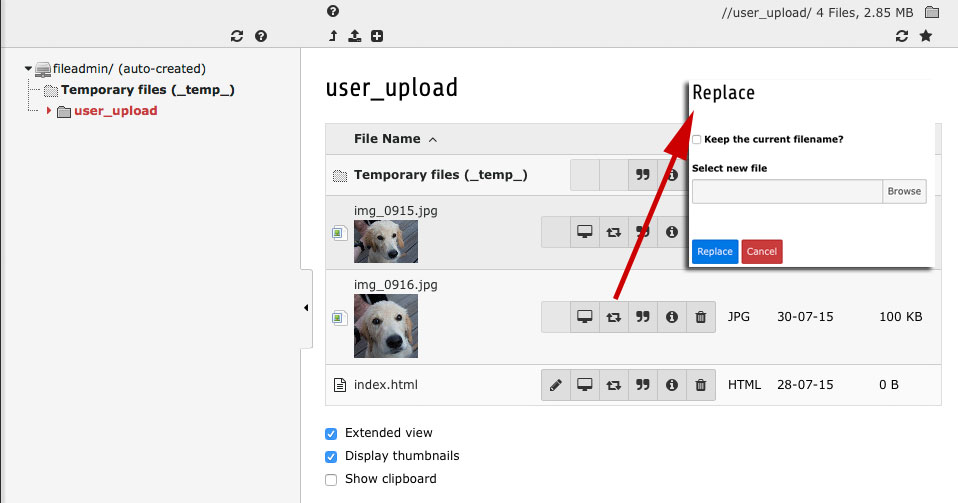
\includegraphics[width=0.75\linewidth]{BackendUserInterface/56133.jpg}
	\end{figure}

\end{frame}

% ------------------------------------------------------------------------------
% LTXE-SLIDE-START
% LTXE-SLIDE-UID:		7a2249dc-f62344bc-c6453178-04b9356d
% LTXE-SLIDE-ORIGIN:	7e5987f7-9a91ea61-8564c721-0f8d5e4a English
% LTXE-SLIDE-ORIGIN:	613354cc-9475feef-bec620c5-31170549 German
% LTXE-SLIDE-TITLE:		Feature: #67574 - Display online status in backend user list
% LTXE-SLIDE-REFERENCE:	Feature-67574-DisplayOnlineStatusInBackendUserList.rst
% ------------------------------------------------------------------------------
\begin{frame}[fragile]
	\frametitle{Backend Gebruikersinterface}
	\framesubtitle{Online-status van Backend-gebruikers}

	De online-status van Backend-gebruikers is te zien in de module "Backend-gebruikers".

	\begin{figure}
		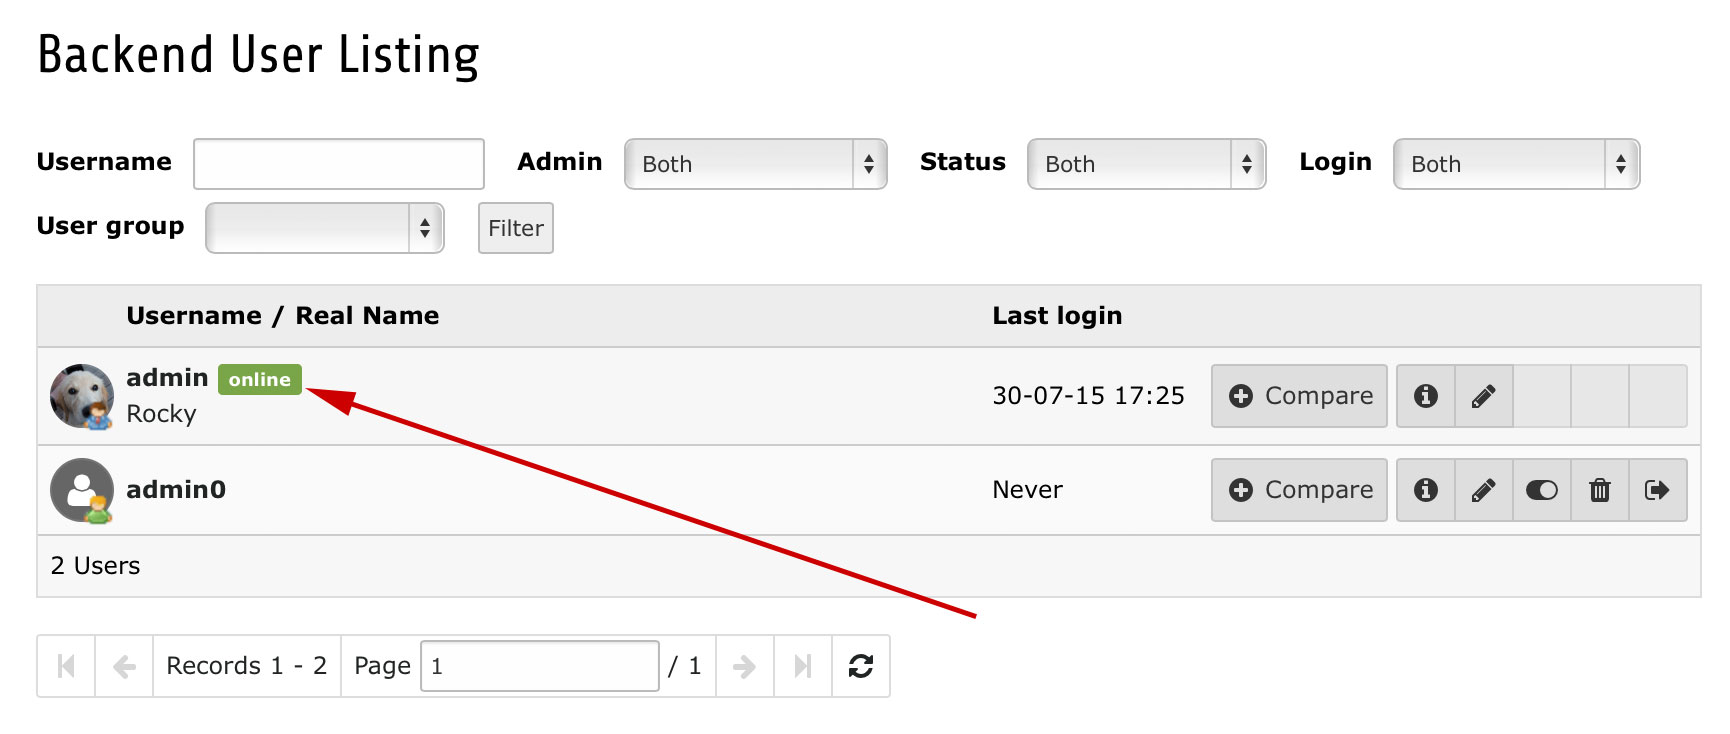
\includegraphics[width=0.9\linewidth]{BackendUserInterface/67574.jpg}
	\end{figure}

\end{frame}

% ------------------------------------------------------------------------------
% LTXE-SLIDE-START
% LTXE-SLIDE-UID:		595b65a9-3e416ac7-882a645c-b55d633d
% LTXE-SLIDE-ORIGIN:	0154fc51-74683590-ebbe8559-ce6a0d57 English
% LTXE-SLIDE-ORIGIN:	00c93fe2-9d128591-20b71814-13556f43 German
% LTXE-SLIDE-TITLE:		FormEngine: Drop "Show secondary options"
% LTXE-SLIDE-REFERENCE:	https://forge.typo3.org/issues/67753
% ------------------------------------------------------------------------------
\begin{frame}[fragile]
	\frametitle{Backend Gebruikersinterface}
	\framesubtitle{Secundaire opties verwijderd}

	Het aanvinkvakje "Secundaire opties tonen (paletten)", de pageTSconfig-optie \texttt{options.enableShowPalettes}
	en de TCA-optie zijn verwijderd. Paletten zijn altijd zichtbaar en kunnen niet verborgen worden.

	\begin{figure}
		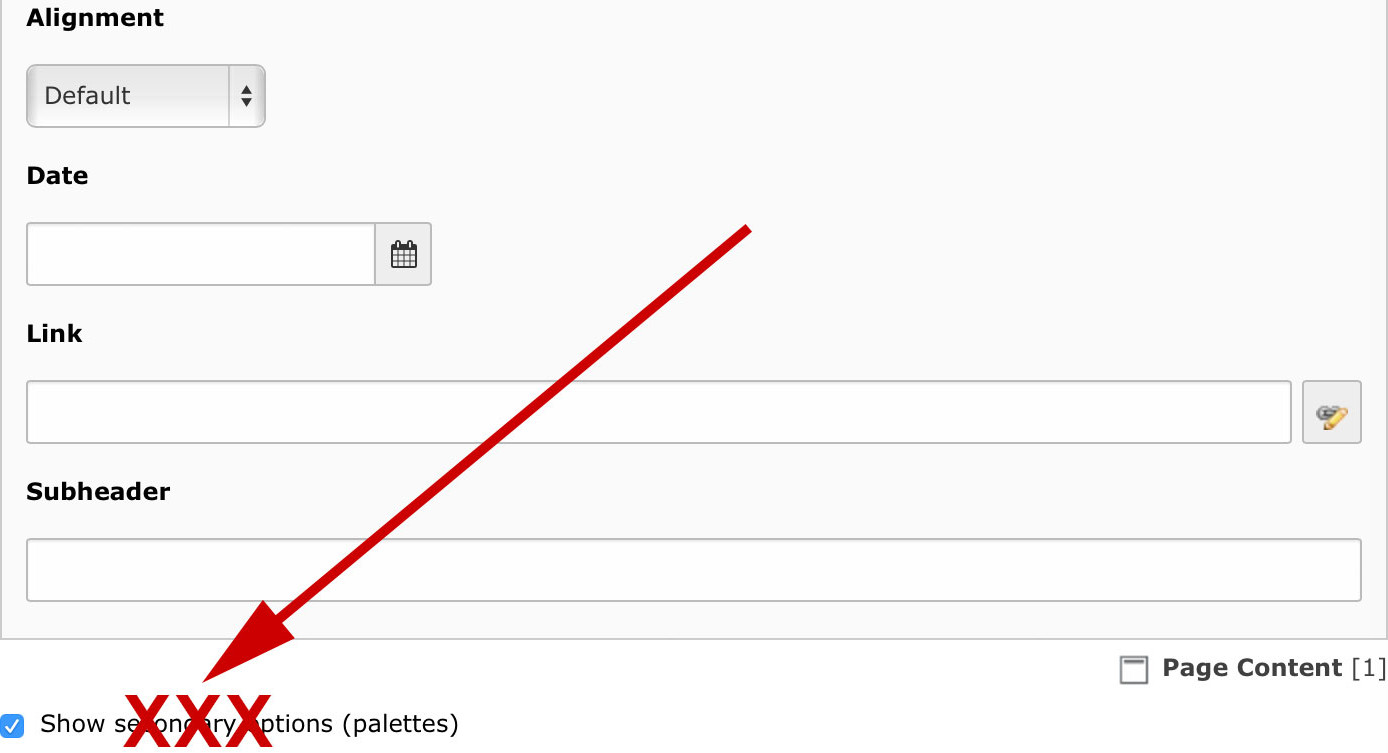
\includegraphics[width=0.7\linewidth]{BackendUserInterface/67753.jpg}
	\end{figure}

\end{frame}

% ------------------------------------------------------------------------------
% LTXE-SLIDE-START
% LTXE-SLIDE-UID:		92615ec2-0fa03590-224642e5-11aa6821
% LTXE-SLIDE-ORIGIN:	f9b24e36-28e8872c-41297de9-52467554 English
% LTXE-SLIDE-ORIGIN:	bab4e93d-0a6d4612-41b2f67e-47c37ff7 German
% LTXE-SLIDE-TITLE:		Feature: #67578 - Add description-field for backend-users
% LTXE-SLIDE-REFERENCE:	Feature-67578-AddDescriptionFieldForBeUsers.rst
% ------------------------------------------------------------------------------
\begin{frame}[fragile]
	\frametitle{Backend Gebruikersinterface}
	\framesubtitle{Beschrijving voor Backend-gebruikers}

	Een nieuw veld "Beschrijving" is toegevoegd aan Backend-gebruikersrecords.

	\begin{figure}
		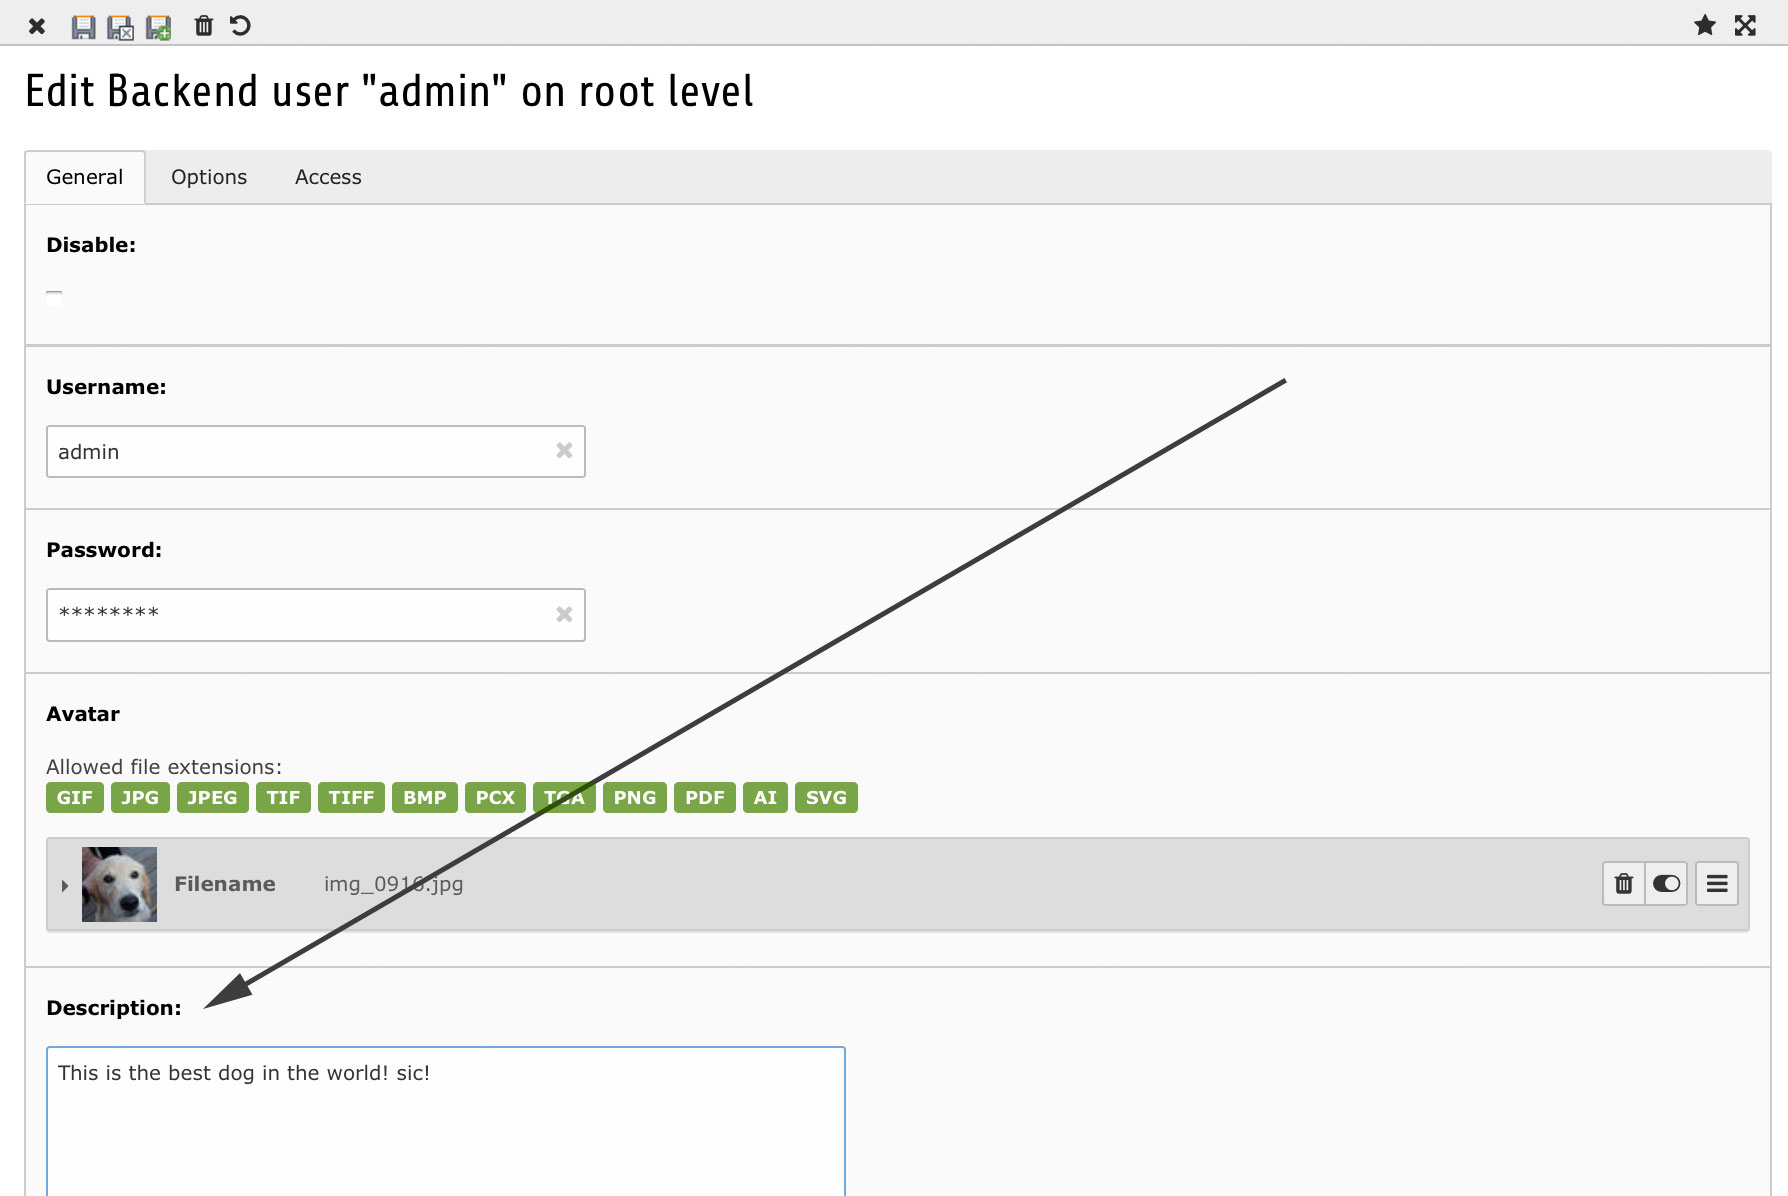
\includegraphics[width=0.7\linewidth]{BackendUserInterface/67578.jpg}
	\end{figure}

\end{frame}

% ------------------------------------------------------------------------------
% LTXE-SLIDE-START
% LTXE-SLIDE-UID:		e3aa82ad-05fde166-7445ba9b-ad75714b
% LTXE-SLIDE-ORIGIN:	83db5442-fa2edfcc-925dd5b6-4afe26f5 English
% LTXE-SLIDE-ORIGIN:	649bd9ee-240381c8-950424ea-f032775b German
% LTXE-SLIDE-TITLE:		Feature: #67603 - Introduce TCA > ctrl > descriptionColumn
% LTXE-SLIDE-REFERENCE:	Feature-67603-IntroduceTcaDescriptionColumn.rst
% ------------------------------------------------------------------------------
\begin{frame}[fragile]
	\frametitle{Backend Gebruikersinterface}
	\framesubtitle{Beschrijving voor tabelkolommen}

	Door een kolom te configureren (meestal \texttt{description}) in de TCA-optie \texttt{['TCA']['ctrl']['descrptionColumn']},
	wordt een beschrijving getoond (handig voor redacteuren en beheerders).

	\begin{figure}
		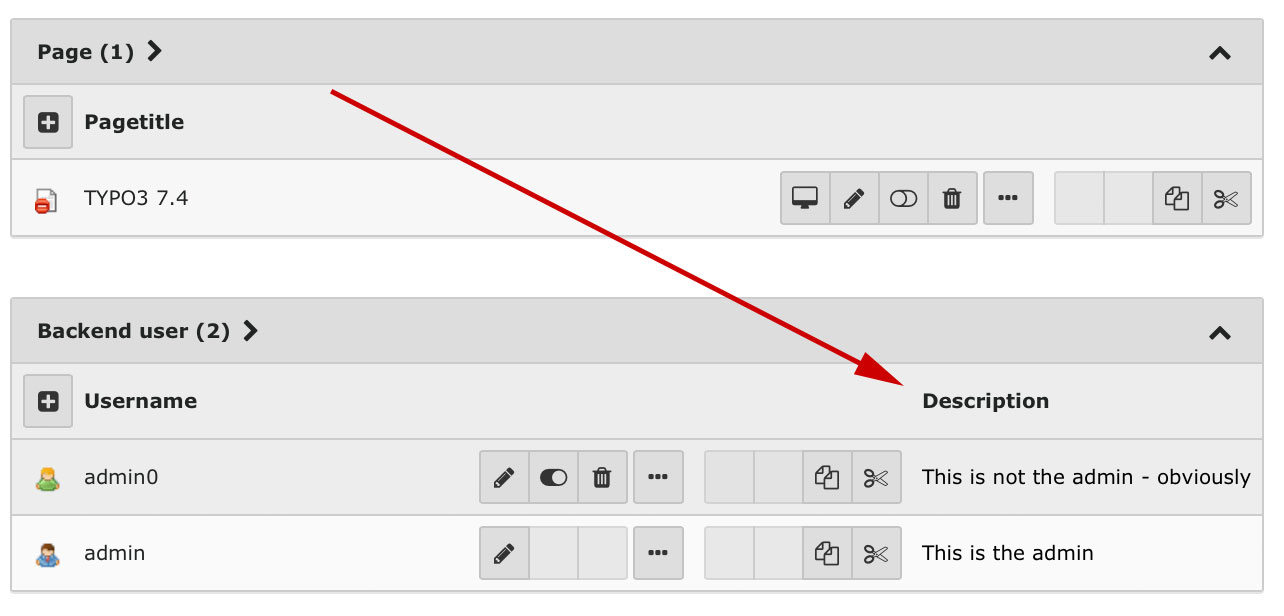
\includegraphics[width=0.7\linewidth]{BackendUserInterface/67603.jpg}
	\end{figure}

\end{frame}

% ------------------------------------------------------------------------------
% LTXE-SLIDE-START
% LTXE-SLIDE-UID:		d15c9433-d0c74450-4deb4f70-e71b1d7f
% LTXE-SLIDE-ORIGIN:	7c5400a9-c4b667f3-1a0c046a-9dd3b6a9 English
% LTXE-SLIDE-ORIGIN:	2eeaec46-1929743b-8e6f9285-13d20d3c German
% LTXE-SLIDE-TITLE:		Feature: #59570 - Add description-field for filemounts
% LTXE-SLIDE-REFERENCE:	Feature-59570-AddDescriptionFieldForFilemounts.rst
% ------------------------------------------------------------------------------
\begin{frame}[fragile]
	\frametitle{Backend Gebruikersinterface}
	\framesubtitle{Beschrijving voor bestandingangen}

	Een nieuw veld "Beschrijving" is toegevoegd aan records voor bestandsingangen.
	Met het veld kunnen beheerders een korte beschrijving toevoegen van het gebruiksdoel van een bepaalde
	bestandsingang, welke documenten het mag bevatten, enz.

	\begin{figure}
		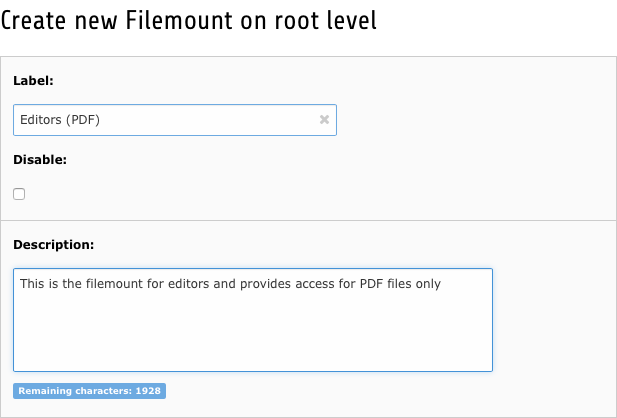
\includegraphics[width=0.55\linewidth]{BackendUserInterface/59570.png}
	\end{figure}

\end{frame}

% ------------------------------------------------------------------------------
% LTXE-SLIDE-START
% LTXE-SLIDE-UID:		bc592063-025c8dd1-b810ba46-f5854146
% LTXE-SLIDE-ORIGIN:	d00f63c4-05272792-21a0a301-4d6a726c English
% LTXE-SLIDE-ORIGIN:	879b1dda-9167d830-373f7457-0391ebee German
% LTXE-SLIDE-TITLE:		Feature: #68197 - Show a dialog for existing files on upload
% LTXE-SLIDE-REFERENCE:	Feature-68197-ShowADialogForExistingFilesOnUpload.rst
% ------------------------------------------------------------------------------
\begin{frame}[fragile]
	\frametitle{Backend Gebruikersinterface}
	\framesubtitle{Dialoog voor bestaande bestanden bij uploaden}

	Als een bestandsupload een bestaand bestand dreigt te overschrijven, wordt een dialoog getoond
	om een actie te kiezen (bijv. vervangen, hernoemen of overslaan).

	\begin{figure}
		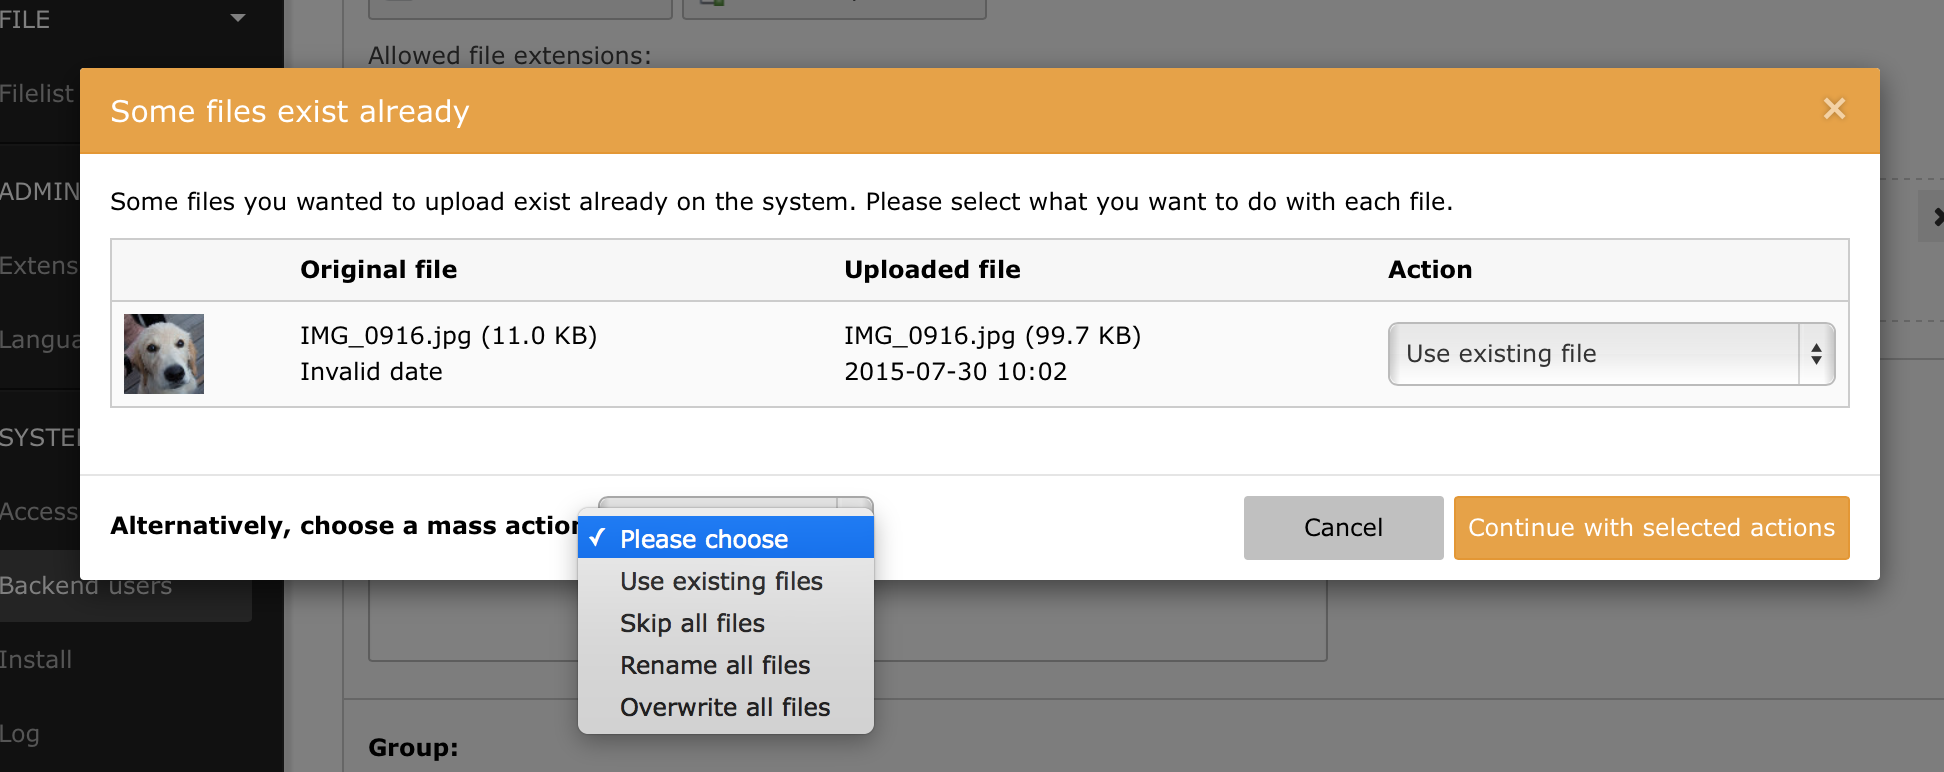
\includegraphics[width=0.9\linewidth]{BackendUserInterface/68197.png}
	\end{figure}

\end{frame}


% ------------------------------------------------------------------------------
% LTXE-SLIDE-START
% LTXE-SLIDE-UID:		5093eb11-2761a299-80509a36-a96ba7fd
% LTXE-SLIDE-ORIGIN:	31d7dd8e-a3c71be4-309850ab-45a7db72 English
% LTXE-SLIDE-ORIGIN:	f4baa7b8-2237ad1d-5c4be365-a845f207 German
% LTXE-SLIDE-TITLE:		Feature: #68218 - Lock edit for tt_content
% LTXE-SLIDE-REFERENCE:	Feature-68218-LockEditForTt_content.rst
% ------------------------------------------------------------------------------
\begin{frame}[fragile]
	\frametitle{Backend Gebruikersinterface}
	\framesubtitle{Beperkt bewerken van inhoudselementen}

	Het bewerken van inhoudselementen kan nu beperkt worden tot alleen beheerders
	(vergelijkbaar met "Beperk bewerken tot beheerders" voor pagina's).

	\begin{figure}
		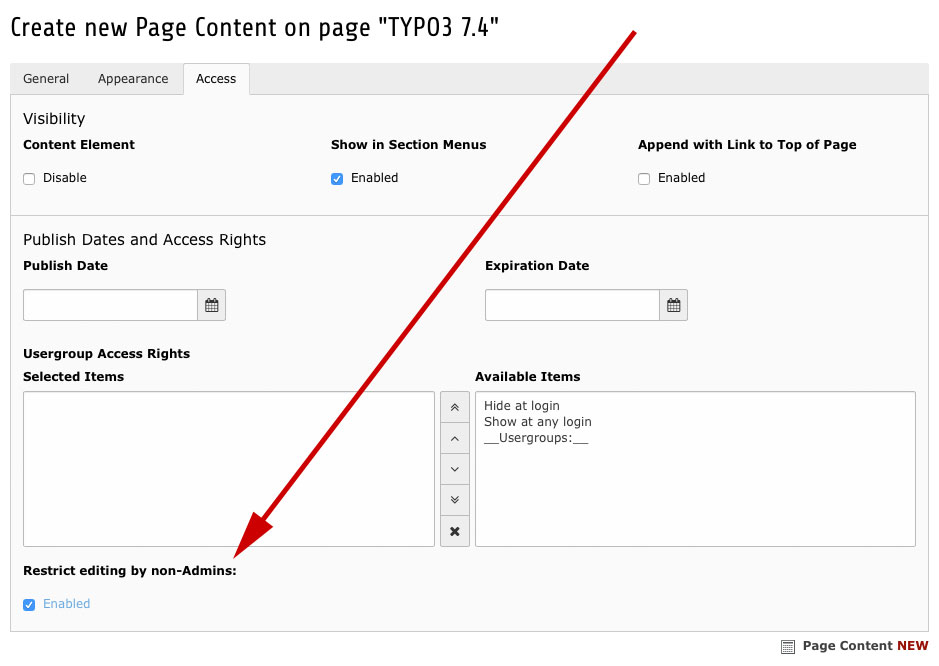
\includegraphics[width=0.6\linewidth]{BackendUserInterface/68218.jpg}
	\end{figure}

\end{frame}

% ------------------------------------------------------------------------------
% LTXE-SLIDE-START
% LTXE-SLIDE-UID:		066bec56-03370f3e-91301316-a5d5f349
% LTXE-SLIDE-ORIGIN:	4e60055a-266e3e24-7baa1613-1226575e English
% LTXE-SLIDE-ORIGIN:	bc83e40f-9b7bac03-ea5f07c4-be27eb56 German
% LTXE-SLIDE-TITLE:		Feature: #68315 - Include pageTSconfig file (1)
% LTXE-SLIDE-REFERENCE:	Feature-68315-IncludeAPageTSconfigFileInPagePropertiesLikeTSStaticTemplates.rst
% ------------------------------------------------------------------------------
\begin{frame}[fragile]
	\frametitle{Backend Gebruikersinterface}
	\framesubtitle{Insluiten Static TSconfig Bestanden (1)}

	Paginaeigenschappen heeft een optie om page TSconfig bestanden in te
	sluiten (zoals dat met TypoScript static templates kan).

	\begin{figure}
		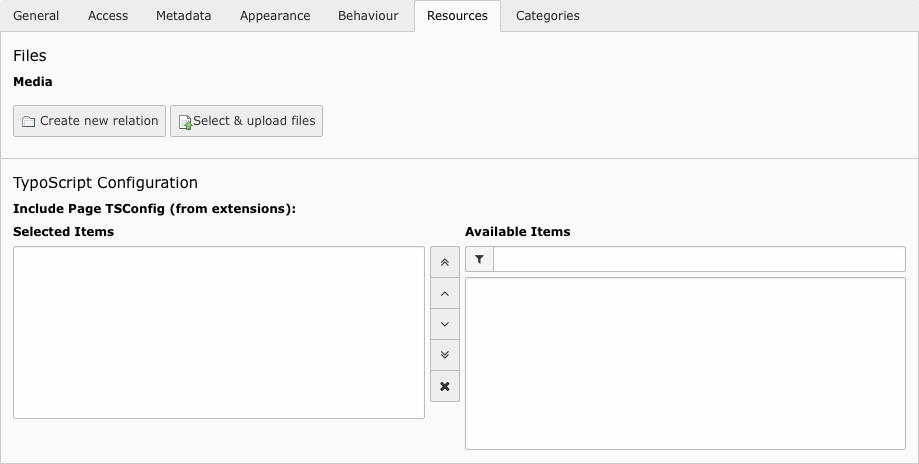
\includegraphics[width=0.8\linewidth]{BackendUserInterface/68315.png}
	\end{figure}

\end{frame}

% ------------------------------------------------------------------------------
% LTXE-SLIDE-START
% LTXE-SLIDE-UID:		0c0383f7-3db2afec-3e89e9e8-33277080
% LTXE-SLIDE-ORIGIN:	4f5cb411-3ea84dfd-84edb16d-433b9fc5 English
% LTXE-SLIDE-ORIGIN:	9b7bac03-ea5f07c4-be27eb56-ac03e27e German
% LTXE-SLIDE-TITLE:		Feature: #68315 - Include pageTSconfig file (2)
% LTXE-SLIDE-REFERENCE:	Feature-68315-IncludeAPageTSconfigFileInPagePropertiesLikeTSStaticTemplates.rst
% ------------------------------------------------------------------------------
\begin{frame}[fragile]
	\frametitle{Backend Gebruikersinterface}
	\framesubtitle{Insluiten Static TSconfig Bestanden (2)}

	% decrease font size for code listing
	\lstset{basicstyle=\tiny\ttfamily}

	De volgende functie registreert een page TSconfig bestand:

	\begin{lstlisting}
		\TYPO3\CMS\Core\Utility\ExtensionManagementUtility::registerPageTSConfigFile(
		  'extensie_naam',
		  'Configuration/PageTS/myPageTSconfigFile.txt',
		  'Mijn speciale configuratie'
		);
	\end{lstlisting}

\end{frame}

% ------------------------------------------------------------------------------
% LTXE-SLIDE-START
% LTXE-SLIDE-UID:		12498449-e1089f75-8654bc4a-6a879644
% LTXE-SLIDE-ORIGIN:	c00b2bfd-2c1b02b0-a7ef9cd0-62f147d2 English
% LTXE-SLIDE-ORIGIN:	f8d888b1-b93dcf4a-e20b976e-9a5c277e German
% LTXE-SLIDE-TITLE:		Feature: #68395 - Allow real copies of content elements into foreign languages
% LTXE-SLIDE-REFERENCE:	Feature-68395-AllowRealCopiesOfContentElementsIntoForeignLanguages.rst
% ------------------------------------------------------------------------------
\begin{frame}[fragile]
	\frametitle{Backend Gebruikersinterface}
	\framesubtitle{Echte kopieën van inhoudselementen}

	Een nieuwe knop in elke kolom van de "Pagina" module zorgt voor \textit{echte} kopieën van inhoudselementen
	naar een taal (niet alleen een referentie).

	\begin{figure}
		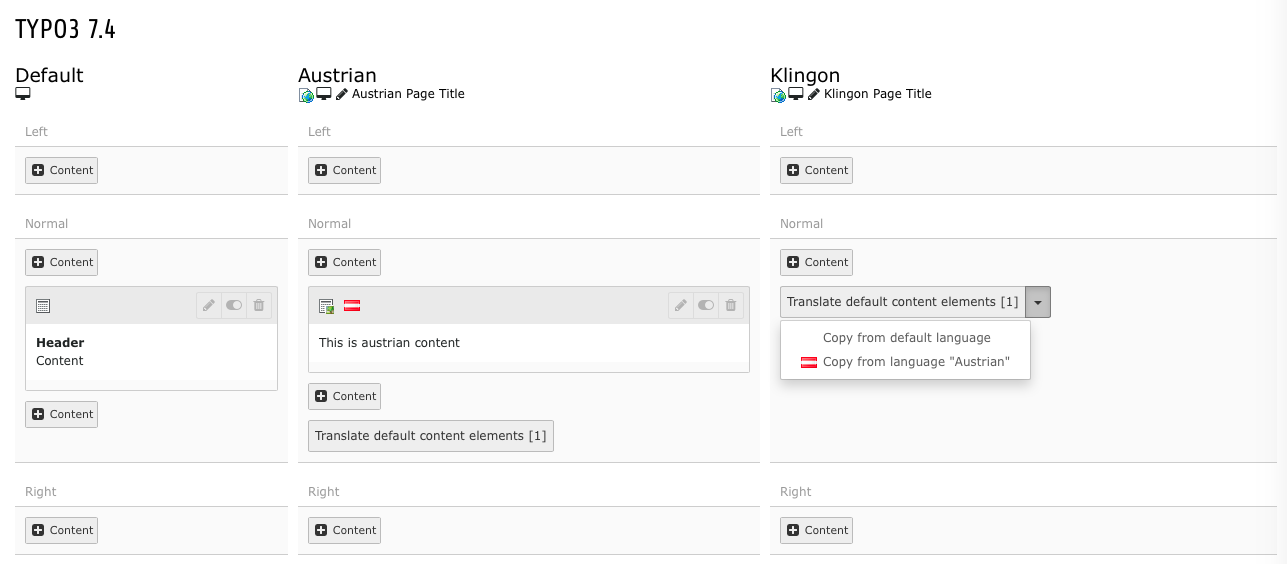
\includegraphics[width=0.9\linewidth]{BackendUserInterface/68395.png}
	\end{figure}

\end{frame}


